% Title: gl2ps_renderer figure
% Creator: GL2PS 1.4.0, (C) 1999-2017 C. Geuzaine
% For: Octave
% CreationDate: Fri Jul 10 23:02:52 2020
\setlength{\unitlength}{1pt}
\begin{picture}(0,0)
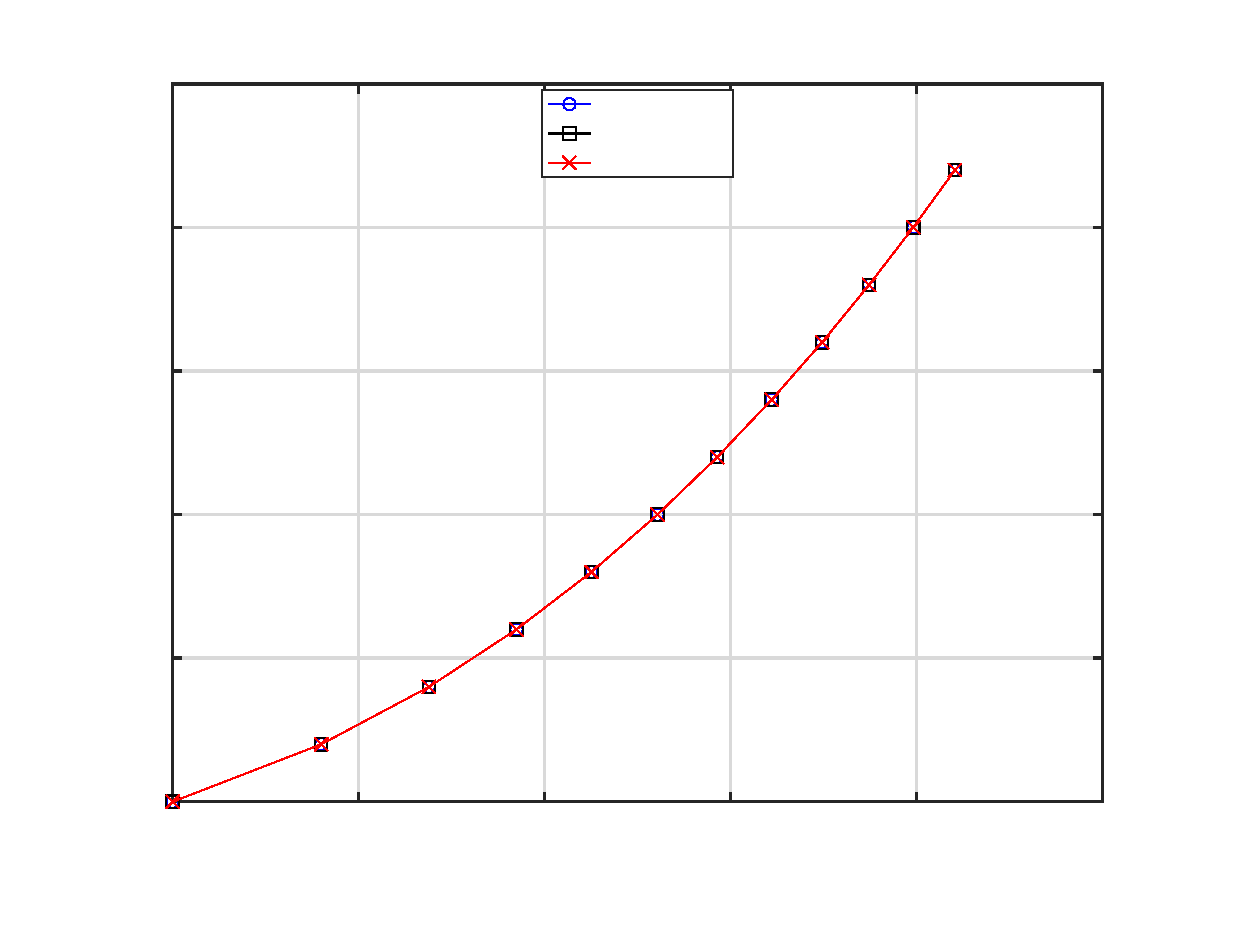
\includegraphics{plotsExtensionSVK-inc}
\end{picture}%
\begin{picture}(576,432)(0,0)
\fontsize{22}{0}
\selectfont\put(74.88,50.0062){\makebox(0,0)[t]{\textcolor[rgb]{0.15,0.15,0.15}{{0}}}}
\fontsize{22}{0}
\selectfont\put(164.16,50.0062){\makebox(0,0)[t]{\textcolor[rgb]{0.15,0.15,0.15}{{0.2}}}}
\fontsize{22}{0}
\selectfont\put(253.44,50.0062){\makebox(0,0)[t]{\textcolor[rgb]{0.15,0.15,0.15}{{0.4}}}}
\fontsize{22}{0}
\selectfont\put(342.72,50.0062){\makebox(0,0)[t]{\textcolor[rgb]{0.15,0.15,0.15}{{0.6}}}}
\fontsize{22}{0}
\selectfont\put(432,50.0062){\makebox(0,0)[t]{\textcolor[rgb]{0.15,0.15,0.15}{{0.8}}}}
\fontsize{22}{0}
\selectfont\put(521.28,50.0062){\makebox(0,0)[t]{\textcolor[rgb]{0.15,0.15,0.15}{{1}}}}
\fontsize{22}{0}
\selectfont\put(69.8755,55.0004){\makebox(0,0)[r]{\textcolor[rgb]{0.15,0.15,0.15}{{0}}}}
\fontsize{22}{0}
\selectfont\put(69.8755,123.92){\makebox(0,0)[r]{\textcolor[rgb]{0.15,0.15,0.15}{{0.5}}}}
\fontsize{22}{0}
\selectfont\put(69.8755,192.84){\makebox(0,0)[r]{\textcolor[rgb]{0.15,0.15,0.15}{{1}}}}
\fontsize{22}{0}
\selectfont\put(69.8755,261.76){\makebox(0,0)[r]{\textcolor[rgb]{0.15,0.15,0.15}{{1.5}}}}
\fontsize{22}{0}
\selectfont\put(69.8755,330.68){\makebox(0,0)[r]{\textcolor[rgb]{0.15,0.15,0.15}{{2}}}}
\fontsize{22}{0}
\selectfont\put(69.8755,399.6){\makebox(0,0)[r]{\textcolor[rgb]{0.15,0.15,0.15}{{2.5}}}}
\fontsize{22}{0}
\selectfont\put(298.08,25.0062){\makebox(0,0)[t]{\textcolor[rgb]{0.15,0.15,0.15}{{Displacement}}}}
\fontsize{22}{0}
\selectfont\put(35.8755,227.3){\rotatebox{90}{\makebox(0,0)[b]{\textcolor[rgb]{0.15,0.15,0.15}{{$\lambda$}}}}}
\fontsize{9}{0}
\selectfont\put(278.373,389.826){\makebox(0,0)[l]{\textcolor[rgb]{0,0,0}{{analytic Sol}}}}
\fontsize{9}{0}
\selectfont\put(278.373,375.767){\makebox(0,0)[l]{\textcolor[rgb]{0,0,0}{{numerical Sol 1}}}}
\fontsize{9}{0}
\selectfont\put(278.373,361.708){\makebox(0,0)[l]{\textcolor[rgb]{0,0,0}{{numerical Sol 2}}}}
\end{picture}
